\documentclass[12pt,a4paper]{article}
\usepackage[utf8]{inputenc}
\usepackage{amsfonts}
\usepackage{amssymb}
\usepackage{graphicx}
\usepackage{float}

% sets margin
\usepackage[hmargin=3cm,vmargin=2.5cm]{geometry}

% creates landscape pages
\usepackage{pdflscape}
\usepackage{pdfpages}

%\renewcommand{\rmdefault}{phv} % Arial
\renewcommand{\sfdefault}{phv} % Arial

% defining settings for textpos
\usepackage[absolute]{textpos}
\setlength{\TPHorizModule}{\paperwidth}
\setlength{\TPVertModule}{\paperheight}

% headers / footers
\usepackage{fancyhdr}
\pagestyle{fancy}
\fancyhf{}
\rhead{Assignment 1}
\lhead{CSG1207: Systems \& Database Design}
\rfoot{\thepage}
\lfoot{Martin Ponce, ID: 10371381}
\renewcommand{\footrulewidth}{0.5pt}

% defining landscape headers / footers
\fancypagestyle{fancylscape}{
	\fancyhf{}
	\renewcommand{\footrulewidth}{0pt}
	\renewcommand{\headrulewidth}{0pt}
	% header
	\begin{textblock}{0.05}[-0.5,-2](0,0)
		{\rotatebox{90}{CSG1207: Systems \& Database Design}}
	\end{textblock}
		\begin{textblock}{0.05}[-0.5,-1](0,0)
		{\rotatebox{90}{Assignment 1}}
	\end{textblock}
	\begin{textblock}{0.05}[-1,-0.109](0,0)
		{\rotatebox{90}{\rule{24.2cm}{0.5pt}}}
	\end{textblock}
	% footer
	\begin{textblock}{0.05}[-19,-4.28](0,0)
		{\rotatebox{90}{Martin Ponce, ID: 10371381}}
	\end{textblock}
		\begin{textblock}{0.05}[-19,-12.8](0,0)
		{\rotatebox{90}{\thepage}}
	\end{textblock}
		\begin{textblock}{0.05}[-18.7,-0.109](0,0)
		{\rotatebox{90}{\rule{24.2cm}{0.5pt}}}
	\end{textblock}
}

% adjusts padding between caption and figure
\setlength{\belowcaptionskip}{10pt}

% adds links to references and colors them blue
\usepackage{hyperref}
\hypersetup{colorlinks=true,
			linkcolor=blue,
			citecolor=black,
			urlcolor=blue}

% apa style referencing
\usepackage[sectionbib, natbibapa]{apacite}
\usepackage{chbibref}

% underlining text
\usepackage[normalem]{ulem}

% \citetapos for possesive citations
\newcommand{\citetapos}[1]{\citeauthor{#1}{\textcolor{black}{'s}} \citeyearpar{#1}}

% add multiline comments \begin{comment} \end{comment}
\usepackage{verbatim}

% front matter
\title{Edith Cowan University\\CSG1207\\Systems \& Database Design\\Assignment 1}
\author{Martin Ponce\\Student 10371381\\\\Tutor: Greg Baatard}
\date{\today}

\begin{document}

% title page
\newpage
\null  % Empty line
\nointerlineskip  % No skip for prev line
\vfill
\let\snewpage \newpage
\let\newpage \relax
\maketitle
\thispagestyle{empty}
\let \newpage \snewpage
\vfill

% toc
\newpage
\tableofcontents
\thispagestyle{fancy}

\newpage
\section{Task 1: Normalisation}

Figure 1 below shows part of a spreadsheet used by a tavern which allows customers to book rooms for events and functions. Each row represents a booking.

\begin{figure}[H]
\centering
\caption{Tavern Bookings}
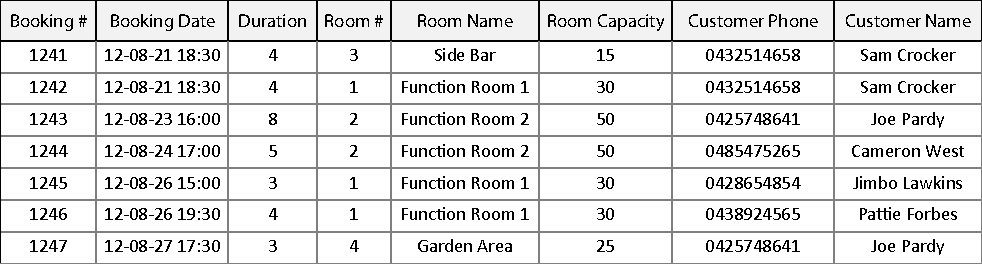
\includegraphics[scale=0.8]{./img/task1.pdf}
\end{figure}

\subsection{Assumptions}

\begin{itemize}
% \item The pub currently identifies customers by their phone number
\item A room cannot have multiple bookings at the same time
\item Auto-incrementing Customer\# has been created, replacing CustomerPhone as customer identifier
	\begin{itemize}
	\item Auto-incrementing identifier avoids user input error which may result in multiple customers with the same phone number
	\item Allows CustomerPhone to be updated without having to update foreign keys if CustomerPhone remained as identifier
	\end{itemize}
\item BookingDate time element has been split into its own attribute
	\begin{itemize}
	\item New attributes created called BookingTimeStart and BookingTimeEnd
	\item Duration attribute is now derived, no longer stored on database
	\item Allows system to check availability of room before a new booking can be created
	\end{itemize}
\end{itemize}

\subsection{0NF: Unnormalised form}

R1 = (Customer\#, CustomerPhone, CustomerName, {Booking\#, BookingDate, BookingTimeStart, BookingTimeEnd, Room\#, RoomName, RoomCapacity})

\subsection{1NF: First normal form}

\sout{R1 = (\textbf{\underline{Customer\#}}, CustomerPhone, CustomerName, \{\textbf{\underline{Booking\#}}, BookingDate, BookingTimeStart, BookingTimeEnd, Room\#,RoomName, RoomCapacity\})}
\\\\
R11 = (\textbf{\underline{Customer\#}}, CustomerPhone, CustomerName)
\\\\
R12 = (\textbf{\underline{Booking\#}}, BookingDate, BookingTimeStart, BookingTimeEnd, Room\#, RoomName, RoomCapacity, \emph{Customer\#})

\subsection{2NF: Second normal form}

No partial dependencies, already 2NF.
\\\\
R11 = (\textbf{\underline{Customer\#}}, CustomerPhone, CustomerName)
\\\\
R12 = (\textbf{\underline{Booking\#}}, BookingDate, BookingTimeStart, BookingTimeEnd, Room\#, RoomName, RoomCapacity, \emph{Customer\#})

\subsection{3NF: Third normal form}

R11 = (\textbf{\underline{Customer\#}}, CustomerPhone, CustomerName)
\\\\
\sout{R12 = (\textbf{\underline{Booking\#}}, BookingDate, BookingTimeStart, BookingTimeEnd, Room\#, RoomName, RoomCapacity, \emph{Customer\#})}
\\\\
R121 = (\textbf{\underline{Booking\#}}, BookingDate, BookingTimeStart, BookingTimeEnd, \emph{Room\#}, \emph{Customer\#})
\\\\
R122 = (\textbf{\underline{Room\#}}, RoomName, RoomCapacity)

\subsection{Named relations}

Customer = (\textbf{\underline{Customer\#}}, CustomerPhone, CustomerName)
\\\\
Booking = (\textbf{\underline{Booking\#}}, BookingDate, BookingTimeStart, BookingTimeEnd, \emph{Room\#}, \emph{Customer\#})
\\\\
Room = (\textbf{\underline{Room\#}}, RoomName, RoomCapacity)

\subsection{Physical E-R diagram}
\newpage
\section{Task 2: Advanced normalisation}

Figure 2 below depicts an invoice for an order from a store.

\begin{figure}[H]
\centering
\caption{Pakoko Tax Invoice}
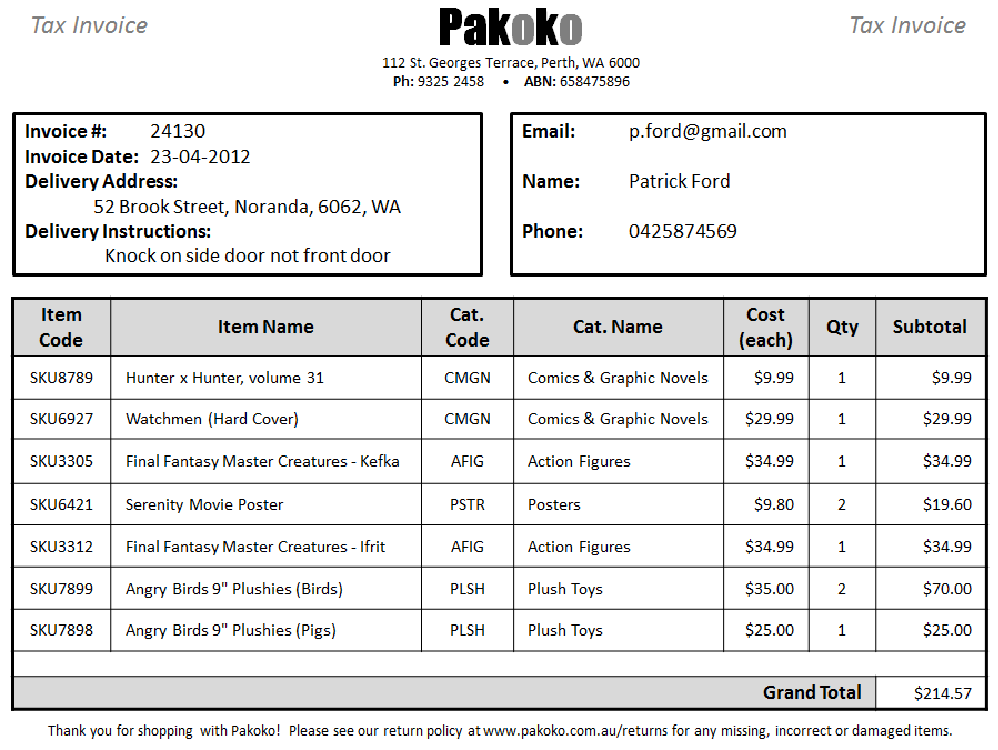
\includegraphics[scale=0.75]{./img/task2.pdf}
\end{figure}

\subsection*{Assumptions}

\begin{itemize}
\item Auto-incrementing Cust\# has been created, replacing CustEmail as customer identifier
	\begin{itemize}
	\item Auto-incrementing identifier avoids user input error which may result in multiple customers with the same email address
	\item Allows CustEmail to be updated without having to update foreign keys if CustEmail remained as identifier
	\end{itemize}
\item Each item is only in one category
\item Item codes are unique per item, even if the items are in different categories
\item Invoice header and footer is static and is not stored in the database
	\begin{itemize}
	\item Includes Pakoko business details header and thank you / return policy URL footer
	\end{itemize}
\item Derived attributes are not stored in the database
	\begin{itemize}
	\item Includes Item Subtotal and Invoice Grand Total
	\end{itemize}
\end{itemize}

\subsection{0NF: Unnormalised form}

R1 = (Cust\#, CustEmail, CustName, CustPhone, DeliveryAddress, DeliveryInstructions, \{Invoice\#, InvoiceDate, \{ItemCode, ItemName, CatCode, CatName, Cost, Qty\}\})

\subsection{1NF: First normal form}

\sout{R1 = (\textbf{\underline{Cust\#}}, CustEmail, CustName, CustPhone, DeliveryAddress, DeliveryInstructions, \{\textbf{\underline{Invoice\#}}, InvoiceDate, \{\textbf{\underline{ItemCode}}, ItemName, CatCode, CatName, Cost, Qty\}\})}
\\\\
R11 = (\textbf{\underline{Cust\#}}, CustEmail, CustName, CustPhone, DeliveryAddress, DeliveryInstructions)
\\\\
R12 = (\textbf{\underline{Invoice\#}}, InvoiceDate, \emph{Cust\#})
\\\\
R13 = (\textbf{\underline{\emph{Invoice\#}}}, \textbf{\underline{ItemCode}}, ItemName, CatCode, CatName, Cost, Qty)

\subsection{2NF: Second normal form}

R11 = (\textbf{\underline{Cust\#}}, CustEmail, CustName, CustPhone, DeliveryAddress, DeliveryInstructions)
\\\\
R12 = (\textbf{\underline{Invoice\#}}, InvoiceDate, \emph{Cust\#})
\\\\
\sout{R13 = (\textbf{\underline{\emph{Invoice\#}}}, \textbf{\underline{ItemCode}}, ItemName, CatCode, CatName, Cost, Qty)}
\\\\
R131 = (\textbf{\underline{\emph{Invoice\#}}}, \textbf{\underline{\emph{ItemCode}}}, Qty)
\\\\
R132 = (\textbf{\underline{ItemCode}}, ItemName, CatCode, CatName, Cost)

\subsection{3NF: Third normal form}

R11 = (\textbf{\underline{Cust\#}}, CustEmail, CustName, CustPhone, DeliveryAddress, DeliveryInstructions)
\\\\
R12 = (\textbf{\underline{Invoice\#}}, InvoiceDate, \emph{Cust\#})
\\\\
R131 = (\textbf{\underline{\emph{Invoice\#}}}, \textbf{\underline{\emph{ItemCode}}}, Qty)
\\\\
\sout{R132 = (\textbf{\underline{ItemCode}}, ItemName, CatCode, CatName, Cost)}
\\\\
R1321 = (\textbf{\underline{ItemCode}}, ItemName, \emph{CatCode})
\\\\
R1322 = (\textbf{\underline{CatCode}}, CatName)

\subsection{Named relations}

Customer = (\textbf{\underline{Cust\#}}, CustEmail, CustName, CustPhone, DeliveryAddress, DeliveryInstructions)
\\\\
Invoice = (\textbf{\underline{Invoice\#}}, InvoiceDate, \emph{Cust\#})
\\\\
InvoiceItem = (\textbf{\underline{\emph{Invoice\#}}}, \textbf{\underline{\emph{ItemCode}}}, Qty)
\\\\
Item = (\textbf{\underline{ItemCode}}, ItemName, \emph{CatCode})
\\\\
Category = (\textbf{\underline{CatCode}}, CatName)

\subsection{Physical E-R diagram}
\section{Task 3: Entity-Relationship modelling}

\subsection{Logical E-R diagram}

\subsection{Physical E-R diagram}
\section{Task 4: Advanced Entity-Relationship modelling}

\subsection{Logical E-R diagram}

\subsection{Physical E-R diagram}

\newpage
\urlstyle{rm}
%\setbibref{\textsf{References}}
\bibliographystyle{apacite}
\addcontentsline{toc}{section}{References}
%\bibliography{./bib/Year 1-Sem 2-CSI1101-A1}

\end{document}